\documentclass[11pt]{article}

\usepackage[letterpaper]{geometry}

\usepackage[utf8]{inputenc} % allow utf-8 input
\usepackage{hyperref}       % hyperlinks
\usepackage{url}            % simple URL typesetting
\usepackage{booktabs}       % professional-quality tables
\usepackage{amsfonts}       % blackboard math symbols
\usepackage{nicefrac}       % compact symbols for 1/2, etc.
\usepackage{microtype}      % micro typography
\usepackage{xcolor}         % colors
\usepackage{tikz}           % drawings
\usepackage{pgfplots}       % plots
\usepackage{xfrac}          % better fractions
\usepackage{amsmath,amsthm,amssymb,bm}
\usepackage{comment,todonotes}
\usepackage{graphicx}
\usepackage[natbib]{biblatex}
\usepackage{fancyhdr,sectsty}
\usepackage{fontspec}
\usepackage{caption,subcaption}
\usepackage{minibox}
\usepackage{parskip,setspace}
\usepackage{epstopdf}
\usepackage[nottoc,numbib]{tocbibind} % Add bibliography to TOC
\usepackage[mathlines]{lineno}

% https://tex.stackexchange.com/questions/461186/how-to-use-lineno-with-amsmath-align

%% Patch 'normal' math environments:
\newcommand*\linenomathpatch[1]{%
  \cspreto{#1}{\linenomath}%
  \cspreto{#1*}{\linenomath}%
  \csappto{end#1}{\endlinenomath}%
  \csappto{end#1*}{\endlinenomath}%
}
%% Patch AMS math environments:
\newcommand*\linenomathpatchAMS[1]{%
  \cspreto{#1}{\linenomathAMS}%
  \cspreto{#1*}{\linenomathAMS}%
  \csappto{end#1}{\endlinenomath}%
  \csappto{end#1*}{\endlinenomath}%
}

%% Definition of \linenomathAMS depends on whether the mathlines option is provided
\expandafter\ifx\linenomath\linenomathWithnumbers
  \let\linenomathAMS\linenomathWithnumbers
  %% The following line gets rid of an extra line numbers at the bottom:
  \patchcmd\linenomathAMS{\advance\postdisplaypenalty\linenopenalty}{}{}{}
\else
  \let\linenomathAMS\linenomathNonumbers
\fi

\linenomathpatch{equation}
\linenomathpatchAMS{gather}
\linenomathpatchAMS{multline}
\linenomathpatchAMS{align}
\linenomathpatchAMS{alignat}
\linenomathpatchAMS{flalign}

\makeatletter
\newcommand\addplotgraphicsnatural[2][]{%
    \begingroup
    % set options in this local group (will be lost afterwards):
    \pgfqkeys{/pgfplots/plot graphics}{#1}%
    % measure the natural size of the graphics:
    \setbox0=\hbox{\includegraphics{#2}}%
    %
    % compute the required unit vector ratio:
    \pgfmathparse{\wd0/(\pgfkeysvalueof{/pgfplots/plot graphics/xmax} - \pgfkeysvalueof{/pgfplots/plot graphics/xmin})}%
    \let\xunit=\pgfmathresult
    \pgfmathparse{\ht0/(\pgfkeysvalueof{/pgfplots/plot graphics/ymax} - \pgfkeysvalueof{/pgfplots/plot graphics/ymin})}%
    \let\yunit=\pgfmathresult
    %
    % configure pgfplots to use it.
    % The \xdef expands all macros except those prefixed by '\noexpand'
    % and assigns the result to a global macro named '\marshal'.
    \xdef\marshal{%
        \noexpand\pgfplotsset{unit vector ratio={\xunit\space \yunit}}%
    }%
    \endgroup
    %
    % use our macro here:
    \marshal
    %
    \addplot graphics[#1] {#2};
}   
\makeatother


\newfontfamily\OpenSans{Open Sans}[Scale=MatchLowercase]
\newfontfamily\SourceSerifPro{Source Serif Pro}[Scale=MatchLowercase,Ligatures=TeX]

%\bibliographystyle{abbrvnat}
\bibliography{biblio.bib}

\pgfplotsset{compat=1.18}
\usetikzlibrary{pgfplots.groupplots,positioning,fit,patterns,decorations.pathreplacing}
\usepgfplotslibrary{fillbetween}


% Margins
\topmargin=-4pt
\evensidemargin=0in
\oddsidemargin=0in
\textwidth=6.5in
\textheight=8.5in
\headsep=0.15in

\onehalfspacing

%\pagestyle{fancy}
%\fancyhf{}
%\lhead{Gaurav Manek}
%\rhead{\thepage}
%\rfoot{\thepage}

\title{ On Value Functions in Temporal Difference Learning }
\author{ Gaurav Manek }  
\date{\today}

\newcommand{\E}{\textbf{E}}
\newcommand{\diag}{\text{diag}}
\newcommand{\tr}{\text{tr}}
\newcommand{\subsectionsubtitle}[1]{\vspace{-0.5em}\textit{#1}\vspace{0.5em}}

% Color Scheme
\definecolor{viridis00}{RGB}{253, 231, 37}
\definecolor{viridis01}{RGB}{181, 222, 43}
\definecolor{viridis02}{RGB}{110, 206, 88}
\definecolor{viridis03}{RGB}{53, 183, 121}
\definecolor{viridis04}{RGB}{31, 158, 137}
\definecolor{viridis05}{RGB}{38, 130, 142}
\definecolor{viridis06}{RGB}{49, 104, 142}
\definecolor{viridis07}{RGB}{62, 73, 137}
\definecolor{viridis08}{RGB}{72, 40, 120}
\definecolor{viridis09}{RGB}{68, 1, 84}

\AddToHook{cmd/section/before}{\clearpage}

\begin{document}

\begin{titlepage}
    {
        \hfill
\includegraphics[width=1.25in,trim=0 0 .125in .25in]{cmu/cmu-wordmark-square-w-on-r}
    }
    \begin{center}{\SourceSerifPro
        \vfill

        {\Huge\OpenSans
            {
                {Stable Models}\\[-1.em]
                \rule{0.25\textwidth}{1pt}
                \raisebox{-.1\baselineskip}{\textit{\Large and}}
                \rule{0.25\textwidth}{1pt}\\[.5em]
                {Temporal Difference Learning}
            }
        }\\


        \vspace{0.25in}

        \textbf{\large Gaurav Manek}\\

        \vfill

        Thesis Proposal

        \textit{In Partial Fulfillment of the Computer Science PhD Program}

        \vspace{0.33in}
        Computer Science Department\\
        School of Computer Science\\
        Carnegie Mellon University\\
        \today

    }\end{center}
\end{titlepage}

\cleardoublepage

~\vfill
\begin{center}
    \begin{minipage}[c]{.7\textwidth}
        \begin{abstract}
            Temporal Difference (TD) learning is used to learn value functions of Markov decision processes (MDPs) using samples following some policy. In Reinforcement Learning (RL), it is necessary to use TD with both function approximation (i.e. neural networks), and off-policy learning. These three conditions are collectively known as the deadly triad because they cause learning to be unstable or diverge. In the literature there are two main strategies to combat this: regularization and reweighting. Our past work has shown the limitations of regularization, and learned reweighting strategies are known to be unstable in practice or have large computational overhead. We have also examined ancilliary strategies that are not effective. We propose POP-TD, a reweighting method based on results from convex optimization that only imposes a constant overhead per iteration.
        \end{abstract}
    \end{minipage}
\end{center}

\vfill

\clearpage

\tableofcontents

\clearpage

\linenumbers

\section{Introduction}

Temporal Difference (TD) learning is used to learn value functions of Markov decision processes (MDPs) using samples following some policy. In Reinforcement Learning (RL), it is necessary to use TD with both function approximation (i.e. neural networks), and off-policy learning. However, these three ingredients are combined, the learned functions exhibit severe instability and divergence. This was first observed by \citet{tsitsiklis1996analysis}, and is known in the literature as the \emph{deadly triad} \cite[p.~264]{sutton2020reinforcement}. While many variants of TD will provably converge despite the training instability, the quality of the solution at convergence is typically arbitrarily poor \citep{kolter2011fixed}.

There are two separate lines of work in the literature that attempt to resolve this: regularization and Emphatic reweighting.
The former attempts to regularize TD, with $\mathcal L_2$-norm weight regularization (common), $\mathcal L_1$ \citep{mahadevan2014proximal}, convex \citep{yu2017convergence}, and bounds propagation \citep{kumar2020discor}.
The second line started with Emphatic-TD, in which \citet{sutton2016emphatic} note that it is possible to reweight samples obtained off-policy so they appear to be on-policy. Such methods learn the follow-on trace using Monte-Carlo methods (in the original) and/or TD \citep{jiang2021learning,zhang2020provably} or techniques similar to TD \citep{hasselt2021expected}.

Current work on deadly-triad-associated training instability is typically evaluated on three standard examples. However, it is possible to regularize training to mitigate divergence in these, and ridge regularization (RR) is used for that in the literature.
In a paper that is in preparation, we introduce a new counterexample (in Figure~\ref{fig:mdp}) that is resistant to regularization. As expected, vanilla TD-based algorithms converge with arbitrarily poor performance for some off-policy distributions ($\eta=0$ line in Figure~\ref{fig:fixedpointp}), and regularization appears to blunt the asymptote ($\eta > 0$ lines). Part of our contribution is that there is a distribution at which the model never performs better than always guessing zeros (i.e. at the limit of RR $\eta\to\infty$) despite any amount of RR, and hence the model is \emph{vacuous}. This problem persists in any algorithm that converges to the same point as naive TD, which covers a wide swath of the extant literature; we make our analysis concrete by showing how this example forces the error bounds derived by \citet{zhang2021breaking} to permit vacuous solutions.

In the same paper, we show how modern Emphatic algorithms that use TD to learn the reweighting function are vulnerable to the bias introduced by RR. These algorithms (near-universally) employ RR so they provably converge despite changing policies. We construct a counterexample in which the emphasis and value models converge correctly when unregularized, but adding regularization causes them to catastrophically diverge.

\todo{Mention MVE. }
\todo{Mention Stable Dynamics Models. }

The focus of our work has now moved on to effectively mitigating this in a manner that is not vulnerable to learning vacuous models or RR-induced bias. We build on the work of \citet{kolter2011fixed}, which derives a condition under which TD is provably stable. Following that work, we have two possible paths. First, we could rewrite the stability criterion so we can compute a closed-form solution for the provably-stable TD update, instead of a nested optimization step. This allows us to reweight updates to be provably stable with only a constant overhead (per iteration) compared to naive TD. Second, we could use Semidefinite Programming (SDP) to compute the reweighting factor for batches of state-transitions. This approach is suitable to larger problems, but we will need to show that the overhead of solving SDPs in the training loop is offset either by better convergence properties or by being able to solve problems that were previously not solvable.

\paragraph{Proposed Thesis Topic:} We propose a novel algorithm to ameliorate the instability from off-policy TD. This algorithm is based on the principles of \cite{kolter2011fixed}, and would work by either (1) computing reweighting factors in a closed-form manner, or (2) by solving an SDP problem for each training minibatch.

\section{Background and Our Work}

The background to the instability is explained by \citet[p.~264]{sutton2020reinforcement}, and the linear case is analyzed in detail by \citet{kolter2011fixed}. The intuition behind this is that the TD fixed point when sampling on-policy is at the solution of the Bellman equation:
\begin{align}
\Phi \vec w & = R + \gamma\,P\,\Phi \vec w
\intertext{for feature basis $\Phi$, learned weights $\vec w$, reward function $R$, discount factor $\gamma$ and transition matrix $P$. However, when TD updates follow an off-policy distribution $\mu\in \mathbb R^n_0$, the TD solution is instead at the fixed point of the Bellman operator followed by a projection:}
\Phi \vec w & = \Pi_\mu \left( R + \gamma P \Phi \vec w \right)
\intertext{where $\Pi_\mu = \Phi (\Phi^\top D \Phi)^{-1} \Phi^\top D$ projects the Bellman backup onto the columnspace of $\Phi$, reweighted by the diagonal matrix $D = \text{diag}(\mu)$. This yields the closed-form solution:}
\vec w & = A^{-1} \vec b
\intertext{Where $A = \Phi^\top D (I - \gamma P) \Phi$ and $\vec b = \Phi^\top D R$. Under ridge regularization, some small $\eta$ is added to the diagonal of $A$ to ensure that the matrix being inverted is positive definite: }
\vec w & = (A + \eta I)^{-1} \vec b \label{eqn:w}
\end{align}
The intuition behind the training instability is that, for some $\mu$, the matrix $A$ is ill-conditioned or singular, causing the inverse to become arbitrarily large or undefined. This training instability occurs even when the bases $\Phi$ can almost exactly represent the value function.

\label{sec:deadlytriadnaive}
\begin{figure}[!p]
  % !TEX root = proposal.tex
\centering
\begin{subfigure}[b]{0.3\textwidth}
  \centering
  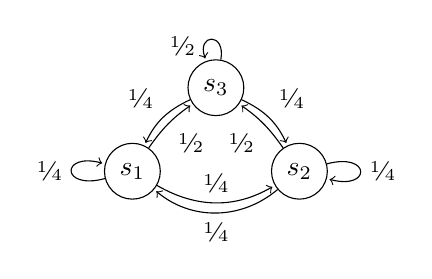
\begin{tikzpicture}[->,shorten >=1pt, node distance={15mm}, main/.style = {draw, circle}] 
    \node[main] (3) {$s_3$}; 
    \node[main] (1) [below left of=3] {$s_1$}; 
    \node[main] (2) [below right of=3]{$s_2$}; 

    \path
    (1) edge[bend left=-30] node[above] {\sfrac 1 4} (2)
        edge[bend right=-10] node[below right] {\sfrac 1 2} (3)
        edge[loop left] node[left] {\sfrac 1 4} (1);

    \path
    (2) edge[bend left=40] node[below] {\sfrac 1 4} (1)
        edge[bend left=-10] node[below left] {\sfrac 1 2} (3)
        edge[loop right] node[right] {\sfrac 1 4} (2);

    \path
    (3) edge[bend left=20] node[above right] {\sfrac 1 4} (2)
        edge[bend right=20] node[above left] {\sfrac 1 4} (1)
        edge[loop above,out=80,in=110,looseness=5] node[left=2mm,pos=0.2] {\sfrac 1 2} (3);

  \end{tikzpicture}
  \caption{Markov Process as a graph.}
  \label{fig:mdp_illustration}

\end{subfigure}
\begin{subfigure}[b]{0.69\textwidth}
  \centering
  \begin{align*}
    \pi = \begin{bmatrix}
      \sfrac 1 4 \\
      \sfrac 1 4 \\
      \sfrac 1 2 \\
    \end{bmatrix}, ~
    \Phi & = \begin{bmatrix}
      1 & 0 \\
      0 & -1 \\
      \sfrac{1}{2} (1.05 + \epsilon) & -\sfrac{1}{2} (1.05 + \epsilon)\\
    \end{bmatrix}, ~
    V = \begin{bmatrix}
      1 \\
      1 \\
      1.05 \\
    \end{bmatrix}
  \end{align*}
  \caption{Stationary distribution $\pi$, Value function basis $\Phi$, True state-values $V$}
  \label{fig:mdp_matrix}
\end{subfigure}

  \caption{Our three-state counter-example MDP. We use this to illustrate how the deadly triad problem persists despite common mitigating strategies. Rewards are set consistent with $V$, and the weights $\vec w$ are trained via TD to minimize $\|\Phi \vec w - V \|$. A small non-zero $\epsilon$ ensures there is some small representation error: $\|\Phi(\Phi^\top \Phi)^{-1}\Phi^\top V - V \| \leq \epsilon$. }
  \label{fig:mdp}
\end{figure}

\paragraph{Reference Example} There are three examples of this TD runaway common in the literature: the classic Tsitsiklis and Van Roy $(w, 2w)$ example \cite[p.~260]{sutton2020reinforcement}, Kolter's example \cite{kolter2011fixed}, and Baird's counterexample which shows how training instability can exist despite overparameterization \cite{baird1993counterexample}. As explained later, these examples are susceptible to regularization, and so we propose our own novel Markov Reward Process (MRP) to illustrate this effect.

Consider the three-state MRP in Figure~\ref{fig:mdp}, with the stationary distribution $\pi$, value function $V$, and value function basis $\Phi$ as indicated. We arbitrarily choose a discount factor $\gamma = 0.99$, and compute the reward function $R \gets (I-\gamma P)V$. The representation error $\|\Pi_D V - V\| \leq \epsilon$ is small by construction.
Closely following the derivation in \cite{kolter2011fixed}, we show that (when $\eta=0$) there is some off-policy distribution $\mu$ such that the error in the value function learned by TD is unbounded. To do this, we set $\mu = [\sfrac p2, \sfrac p2, 1-p]$ to be a sampling distribution parameterized by $p \in [0..1]$ and find a value of $p$ around which the matrix $A$ is ill-conditioned. Solving $\det(A) = 0$, we obtain:
\begin{align}
  p & = \frac{40400\epsilon^2 + 45240\epsilon + 2961}{40400\epsilon^2 + 84840\epsilon + 4141}\label{eqn:simplep}
\end{align}
Since this solution is in the range $[0, 1]$ for all positive $\epsilon$, there is always some sampling distribution parameter $p$ at which $A$ is ill-conditioned, and hence $A^{-1}$ can be made arbitrarily large by selecting a point close to $p$. We can therefore obtain any error, which completes this introductory example.

We plot the relationship between TD error and $p$ in Figure~\ref{fig:fixedpointp}. The two key features of this are: first, the error is smallest when the sampling distribution $\mu$ is close to the stationary distribution $\pi$ close to $p=0.5$. Second, the error only asymptotically diverges at specific off-policy distributions, notably at about $p=0.715$. It remains low everywhere else.

%%
\begin{figure}[!p]
    \begin{tikzpicture}
    \begin{axis}[
        scale only axis,
        width=\textwidth-10mm,
        height=5cm,
        tick align=outside,
        enlargelimits=false,
        ymode=log,
        mark=none,
        ymax=10,
        xlabel={$p$ in sampling distribution $\mu=[\sfrac p2, \sfrac p2, 1-p]$},
        yticklabels={,,},
        ylabel={TD error},
    ]
    \addplot[color=viridis09,thick] table [x=p, y=err] {fixedpointp/eta_-infty.dat} node[below,pos=0.002] {$\eta=0$};
    \addplot[color=viridis03] table [x=p, y=err] {fixedpointp/eta_-6.dat} node[above,pos=0.01] {$\eta=10^{-6}$};
    \addplot[color=viridis03] table [x=p, y=err] {fixedpointp/eta_-4.dat} node[above,pos=0.022] {$\eta=10^{-4}$};
    \addplot[color=viridis03] table [x=p, y=err] {fixedpointp/eta_-2.dat} node[below,pos=0.1] {$\eta=10^{-2}$};
    \addplot[color=black,thick,dashed] table [x=p, y=err] {fixedpointp/eta_infty.dat} node[above,pos=0.06] {$\eta\to\infty$};
    \end{axis}
\end{tikzpicture}

    \caption{We plot TD error against $p$ for the MDP in Figure~\ref{fig:mdp} with $\epsilon=10^{-4}$. This shape is characteristic of TD models in the presence of the deadly triad, including a minima close to $\pi$ ($p=0.5$), and an asymptote at the singular point ($p\approx 0.715$). At different levels of regularization the error function moves between the unregularized case ($\eta=0$) and the limiting case ($\eta\to\infty$).}
    \label{fig:fixedpointp}
\end{figure}
%%

%%%%%%%%%%%%%%%%%%%%%%%%%%%%%%%%%%%%%%%%%%%%%%%%%%%%%%%%%%%%
This is a well-known problem in the literature with many training strategies developed for it, both theoretical and practical. We select some key strategies for discussion here.

\subsection{Ridge Regularization}
\subsectionsubtitle{Contains work from \cite{manek2022pitfalls}: \citetitle{manek2022pitfalls}~(\citeauthor{manek2022pitfalls},~\citeyear{manek2022pitfalls})}
\label{sec:rr}

One classic solution to this problem is to adopt some sort of regularization to avoid unbounded error or divergence. \emph{Ridge regularization} (RR) \cite{tikhonov1943stability} is the most popular regularization strategy by far, which is generally understood to bound the worst-case error in exchange for biasing the model and potentially increasing the error everywhere else. RR works by penalizing the $\mathcal L_2$-norm of model weights, which limits the scale of the predicted values and the model output. When used to evaluate the deadly triad on three common examples \cite[pg.260]{kolter2011fixed,baird1993counterexample,sutton2020reinforcement}, RR appears to be able to effectively mitigate the worst of the divergence. Consequently, it has become an essential assumption made by many RL algorithms \cite{diddigi2019convergent,mahadevan2014proximal,sutton2009fast,yu2017convergence,zhang2020provably,zhang2021breaking} and is viewed in the literature as a routine and innocuous assumption. Our previous work \citep{manek2022pitfalls} challenges that assumption by introducing counterexamples that shows that training instability is \emph{not} solved by the use of RR.

\subsubsection{RR admits vacuous models}
Instead of using asymptotic error as a measure of divergence, we define a \emph{vacuous model} as one that, for all $\eta$, never performs better than the limiting error at $\eta\to\infty$. (At the limit $\eta\to\infty$, all model weights are zero and so is the model output.) Intuitively, a vacuous model is one that never does better than always predicting zeros.

Even though RR \emph{appears} to mitigate the training instability, it merely hides it. This can be observed in Figure~\ref{fig:fixedpointp}, which illustrates the effect of RR on the error landscape in our three-state MRP. While RR blunts the asymptote, it increases the error everywhere quickly enough that there is some off-policy distribution under which TD learns always learns a vacuous model despite any amount of regularization. In previous work \citep{manek2022pitfalls}, we identified the exact point and proved this.

\todo{Add more explanation here. }

\subsubsection{RR and small-eta divergence}
Further, there is a general assumption in the literature that RR monotonically shrinks the learned weights and model output. While this is true in classification, regression, and other non-bootstrapping contexts this is \emph{not} true in TD. Because TD repeatedly bootstraps values it is possible for small amounts of model bias to be magnified and induce model divergence.
From Equation~\ref{eqn:w}, we can see that RR ensures the matrix $(A + \eta I)$ is positive definite and therefore invertible without blowing up. This is necessary because, under off-policy distributions, it is possible for $A$ to have eigenvalues that are negative or zero.

In the literature, it is commonly assumed that $A$ is ``nearly'' positive definite (that is, only a few eigenvalues are non-positive, and those are close to zero.). One interpretation of RR is that it increases those eigenvalues to ensure the matrix $(A + \eta I)$ is positive definite. However, adding just the right value of $\eta$ can move these negative eigenvalues arbitrarily close to zero, inducing a correspondingly large bias.
This small-$\eta$ divergence effect can appear in several ways, illustrated in Figure~\ref{fig:etagraph}. Typically, this appears as one or more points at which TD error diverges at some $\eta$ before the region at which RR ``improves'' the model (that is, reduces the model error below $\|V\|$). This suggests that by setting a lower bound $\eta_0$ we can guarantee that $(A + \eta I)$ is positive definite for all $\eta > \eta_0$. The third example in Figure~\ref{fig:etagraph} contradicts this intuition: increasing RR to an improved model can also make it diverge. If we set $\eta_0$ to prohibit divergence, the resultant model is vacuous.

\begin{figure}[p]
  \begin{subfigure}[t]{0.48\textwidth}
    \centering
    

\begin{tikzpicture}
    \begin{groupplot}[
        group style={
            group size=1 by 3,
            x descriptions at=edge bottom,
            vertical sep=0pt,
        },
        scale only axis,
        width=\textwidth-8mm,
        height=2cm,
        tick align=outside,
        enlargelimits=false,
        xmin=0.000000001,
        xmax=1,
        xmode=log,
        xlabel={RR parameter $\eta$},
        x tick label style={font=\small, yshift=0.5ex},
        xtick align=inside,
        xtick={0.000000001, 0.000001, 0.001, 1},
    ]


    \nextgroupplot[
        mark=none,
        ymax=10000,
        ymin=0.05,
        ymode=log,
        yticklabels={,,},
        ytick style={draw=none},
    ]
    \node[anchor=south east,black] at (axis cs:.8, 2.25) {$\scriptstyle \|V\|$};
    \draw[dashed,very thick,gray] (axis cs:0.000000001, 2.25) to[] (axis cs:1000, 2.25);

    %\node[anchor=north east,black] at (axis cs:.8, 0.044) {$\epsilon$};
    %\draw[dashed,very thick,gray] (axis cs:0.000000001, 0.044) to[] (axis cs:1000, 0.044);

    \addplot[color=viridis06,thick] table [x=eta, y=err] {smalleta/data/td_smalleta_B.dat};


    \nextgroupplot[
        mark=none,
        ymax=10000,
        ymin=0.05,
        ymode=log,
        yticklabels={,,},
        ytick style={draw=none},
        ylabel={TD error},
        ylabel style={yshift=-3mm},
    ]
    \node[anchor=south east,black] at (axis cs:.8, 2.25) {$\scriptstyle \|V\|$};
    \draw[dashed,very thick,gray] (axis cs:0.000000001, 2.25) to[] (axis cs:1000, 2.25);

    %\node[anchor=north east,black] at (axis cs:.8, 0.044) {$\epsilon$};
    %\draw[dashed,very thick,gray] (axis cs:0.000000001, 0.044) to[] (axis cs:1000, 0.044);

    \addplot[color=viridis03,thick] table [x=eta, y=err] {smalleta/data/td_smalleta_A.dat};


    \nextgroupplot[
        mark=none,
        ymax=1000,
        ymin=0.0001,
        ymode=log,
        yticklabels={,,},
        ytick style={draw=none},
    ]
    \node[anchor=north east,black] at (axis cs:.8, 2.25) {$\scriptstyle \|V\|$};
    \draw[dashed,very thick,gray] (axis cs:0.000000001, 2.25) to[] (axis cs:1000, 2.25);

    %\node[anchor=north east,black] at (axis cs:.8, 0.044) {$\epsilon$};
    %\draw[dashed,very thick,gray] (axis cs:0.000000001, 0.044) to[] (axis cs:1000, 0.044);

    \addplot[color=viridis09,thick] table [x=eta, y=err] {smalleta/data/td_smalleta_C.dat};

    \end{groupplot}
\end{tikzpicture}

    \vspace{-1.25em}
    \caption{Different MPs at off-policy distributions selected to show small-$\eta$ divergence. Divergence may occur at multiple $\eta$, and may even occur \emph{after} the $\eta$ that minimizes TD error. }
    \label{fig:etagraph}
  \end{subfigure}
  \hfill
  \begin{subfigure}[t]{0.48\textwidth}
    \centering
    \begin{tikzpicture}
    \begin{axis}[
        scale only axis,
        width=\textwidth-10mm,
        height=3.99cm,
        tick align=outside,
        enlargelimits=false,
        mark=none,
        ymax=100,
        ymin=0.01,
        ymode=log,
        xmin=0.000000001,
        xmax=0.1,
        xmode=log,
        xlabel={RR parameter $\eta$},
        %ylabel={TD error},
        x tick label style={font=\small, yshift=0.5ex},
        y tick label style={font=\small, xshift=0.5ex},
        ytick align=inside,
        xtick align=inside,
        xtick={0.000000001, 0.000001, 0.001, 1},
    ]

    \node[anchor=south east,black] at (axis cs:.08, 2.25) {$\|V\|$};
    \draw[dashed,very thick,gray] (axis cs:0.000000001, 2.25) to[] (axis cs:1000, 2.25);

    \node[anchor=north east,black] at (axis cs:.08, 0.044) {$\epsilon$};
    \draw[dashed,very thick,gray] (axis cs:0.000000001, 0.044) to[] (axis cs:1000, 0.044);


    \addplot[color=viridis03,thick] table [x=eta, y=err] {fixedpointeta/data/td_eta_A.dat};
    \draw[dotted,very thick,viridis03!50] (axis cs:0.000000053088, 0.00001) to[] (axis cs:0.000000053088, 0.1748);

    \addplot[color=viridis06,thick] table [x=eta, y=err] {fixedpointeta/data/td_eta_B.dat};
    \draw[dotted,very thick,viridis06!50] (axis cs:0.0001258, 0.00001) to[] (axis cs:0.0001258, 1.2431);

    \addplot[color=viridis09,thick] table [x=eta, y=err] {fixedpointeta/data/td_eta_C.dat};
    \draw[dotted,very thick,viridis09!50] (axis cs:0.00000237137, 0.00001) to[] (axis cs:0.00000237137, 0.23783);

    \end{axis}
\end{tikzpicture}

    \vspace{-1.25em}
    \caption{Three off-policy distributions for a five-state MP, with mutually incompatible $\eta$. The optimal $\eta$ for any one distribution strongly over- or under-regularizes the error at the other distributions. }
    \label{fig:mismatchedeta}
  \end{subfigure}
    \caption{We plot TD error against $\eta$ to show small-$\eta$ divergence (left) and mututally-incompatible $\eta$ (right). We also plot the error at the limit of RR $\|V\|$ and the representation error $\epsilon$. }
\end{figure}

\paragraph{In Neural Networks} We emphasize that this is not just an theoretical concern--we demonstrate this in the neural network case using a 9-state variant of our example. We randomly assign a value function and train 100 randomly-initialized models to convergence, plotting the mean and the $10^\text{th}$--$90^\text{th}$ percentile range in Figure~\ref{fig:multilayerperformance} (left), with and without RR. 
Because we are now working with neural networks and not linear models TD is able to learn models without asymptotes. Since we cannot use asymptotic error to diagnose model divergence, we instead assume that models that perform worse than guessing zero have diverged. Figure~\ref{fig:multilayerperformance} plots this threshold ($\|V\|_2$, dashed grey line). We observe that despite regularization our models perform worse than guessing zero under some off-policy distributions, notably in the domain $p\in[0.1, 0.4]$. This shows that training instability from off-policy learning carries over to the neural network case.

We also plot the TD error against the RR parameter $\eta$ at a fixed off-policy distribution (Fig.~\ref{fig:multilayerperformance}, right). We observe that around $\eta\approx 10^{-3}$ the TD Error unexpectedly \emph{increases} before decreasing. The classic intuition of how ridge regularization works is that it monotonically crushes model parameters (and hence predictions) towards zero, but because TD learns by bootstrapping, the same intuition does not carry over.

\begin{figure}
  \centering

\begin{tikzpicture}
    \begin{axis}[
    width=0.5\textwidth,
    height=0.3\textwidth,
    ymin=0.01,
    ymax=10,
    ymode = log,
    xmin=0,
    xmax=1,
    title = {TD Error over Distributions},
    xlabel={Distribution parameter $p$},
    xtick={0,0.2,0.4,0.6,0.8},
    legend style={legend cell align=left, legend pos=south west,nodes={scale=0.75, transform shape}},
    ]
        \addplot[dashed,color=black] table [x=p, y=v0err] {multilayerperf/basic.dat}
            node[below,pos=0.2] {$\|V\|_2$};

        \addplot[color=red,very thick] table [x=p, y=mean] {multilayerperf/dump_3_0.dat};
        \addplot[color=red,very thin,name path=lcb,] table [x=p, y=conf_05] {multilayerperf/dump_3_0.dat};
        \addplot[color=red,very thin,name path=ucb,] table [x=p, y=conf_95] {multilayerperf/dump_3_0.dat};
        \addplot[pattern=crosshatch,pattern color=red!50,area legend] fill between[of=lcb and ucb];

        \addplot[color=blue,very thick] table [x=p, y=mean] {multilayerperf/dump_3_0.001.dat};
        \addplot[color=blue,very thin,name path=lcb,] table [x=p, y=conf_05] {multilayerperf/dump_3_0.001.dat};
        \addplot[color=blue,very thin,name path=ucb,] table [x=p, y=conf_95] {multilayerperf/dump_3_0.001.dat};
        \addplot[blue!15,area legend] fill between[of=lcb and ucb];

        \legend{,,,,unregularized,regularized}
    \end{axis}
\end{tikzpicture}
\begin{tikzpicture}
    \begin{axis}[
    width=0.5\textwidth,
    height=0.3\textwidth,
    ymin=2.0,
    ymax=4.0,
    xmin=0.00001,
    xmax=1,
    title = {TD Error vs $\eta$ at $p=0.31$},
    xlabel={RR parameter $\eta$},
    xmode=log,
    ]
        \addplot[color=blue,very thick] table [x=eta, y=mean] {multilayerperf/etas_p_0.31.dat};
        \addplot[color=blue,very thin,name path=lcb,] table [x=eta, y=conf_05] {multilayerperf/etas_p_0.31.dat};
        \addplot[color=blue,very thin,name path=ucb,] table [x=eta, y=conf_95] {multilayerperf/etas_p_0.31.dat};
        \addplot[blue!15] fill between[of=lcb and ucb];

        \addplot[dashed,color=black] table [x=eta, y=v0err] {multilayerperf/basic.dat};
    \end{axis}
\end{tikzpicture}

  \caption{On the left we present the mean and $10^\text{th}$--$90^\text{th}$ percentile range of 100 randomly-initialized NN models trained to convergence. On the right we present the relationship between error and the RR parameter $\eta$ at a specific off-policy distribution. We annotate both charts with $\|V\|_2$, which corresponds to the error from guessing zeros. }
  \label{fig:multilayerperformance}
\end{figure}

\subsubsection{RR and mutually-incompatible parameters}

The best value of $\eta$ depends strongly on the specific off-policy distribution. Selecting a single value that doesn't diverge over all training distributions can lead to values that strongly over-regularize over most distributions. We illustrate this in Figure~\ref{fig:mismatchedeta}, which plots the TD error over $\eta$ for three different off-policy distributions. In this plot, selecting an $\eta$ that minimizes the error at any one distribution will lead to poor or vacuous results in the other two distributions.
Further complicating this is the use of RR to permit slow distribution change during training, as described in the next section. If the training distribution changes while $\eta$ is fixed then formerly convergent TD may diverge.

\subsubsection{In the literature}

To show that relying on RR is a risky decision to make, we further analyzed our three-state MRP example in the context of the algorithm in \citetitle{zhang2021breaking} \citep{zhang2021breaking}. In that paper, the authors assume the use of RR to derive bounds on the learned error under off-policy sampling. We are able to show that their bounds are very loose on our example, permitting vacuous models.

Ridge regularization is particularly common when proving that some training method converges despite a changing sampling policy. This is seen in GTD (analyzed in \cite{yu2017convergence}), GTD2 \cite{sutton2009fast}, RO-TD \cite{mahadevan2014proximal}, and COF-PAC \cite{zhang2020provably}. This assumption may also be used to ensure convergence when training with a target network \cite{zhang2021breaking}. Despite the prevalence of ridge regularization, the induced bias from using it is not well studied in the literature. It is sometimes even dismissed as a mere technical assumption, as in \cite{diddigi2019convergent}. A key conclusion of our prior work contradicts that; using ridge regularization for convergence proofs induces bias that may hinder performance.

RR penalizes the $\mathcal L_2$-norm of the learned weights; it is also possible to use $\mathcal L_1$ regularization with a proximal operator/saddle point formulation as in \cite{mahadevan2014proximal}, or any convex regularization term under a fixed target policy \cite{yu2017convergence}. Instead of directly regularizing the weights, COP-TD uses a discounted update \cite{gelada2019off}. DisCor \cite{kumar2020discor} propagates bounds on Q-value estimates to quickly converge TD learning in the face of large bootstrapping error; it is not clear if DisCor can overcome off-policy sampling. A separate primal-dual saddle point method has also been adapted to ridge regularization \cite{du2017stochastic} and is known to converge under deadly triad conditions, error bounds of this convergence are not yet known.


\subsection{Emphatic-TD Style Algorithms}
\subsectionsubtitle{Contains work from \cite{manek2022pitfalls}: \citetitle{manek2022pitfalls}~(\citeauthor{manek2022pitfalls},~\citeyear{manek2022pitfalls})}

Emphatic-TD \cite{sutton2016emphatic} fixes the fundamental problem in off-policy TD by reweighing updates so they appear on-policy. The core idea underlying these techniques is to estimate the ``followon trace'' for each state, the (weighted, $\lambda$- and $\gamma-$discounted) probability mass of all states whose value estimates it influences. This trace is then used to estimate the emphasis, which is the reweighting factor for each update. While this family of methods is provably optimal in expectation, it is subject to tremendous variance in theory and practice, especially when the importance is estimated using Monte-Carlo sampling.\footnote{Sutton and Barto's textbook \citeyearpar{sutton2020reinforcement} says about Emphatic-TD that ``it is
nigh impossible to get consistent results in computational experiments.'' (when applied to Baird's example). } 
There is considerable interest in making this more practical, especially by learning the importance and value models simultaneously.

A leading example of this work is COF-PAC \cite{zhang2020provably}, which uses ridge regularized versions of GTD2 \cite{sutton2009fast} to learn an emphasis model while using that model to also learn a value function. The authors describe RR as essential to their method, particularly when the target policy changes during learning. This reliance on RR makes COF-PAC (and most other TD-based Emphatic algorithms) vulnerable to model bias.
We illustrate this with a counterexample in which COF-PAC diverges because of its reliance on RR.
To generate this counterexample, we apply our three-state MRP to COF-PAC, choosing to learn the value function at the off-policy distribution correponding to $p=0.4$. From Figure~\ref{fig:fixedpointp} we can see that $p=0.4$ lies in the stable region of the error landscape, and so regular TD will converge to a reasonable solution; however, we show how COF-PAC diverges.

COF-PAC has two main parts, an emphasis function and a value function. At each TD update, the emphasis function is updated and then used to reweight incoming value functions. A convenient way to conceptualize COF-PAC is to think in terms of the ``effective'' distribution $\upsilon(\eta)$ (that is, the net distribution after correction.) This depends on (1) the sampling distribution ($\mu$), (2) the regularization applied to the emphasis model during learning, and (3) the target distribution of the correction, typically $\pi$.

In Figure~\ref{fig:emphimpetam} plot the distance between the effective distribution $\upsilon(\eta)$ and the target distribution $\pi$ for our example. The unregularized distribution error is low, but adding RR greatly increases the distance between the effective and target distributions.
Without regularization, COF-PAC will resample input so it appears to be on-policy and the value function will converge to a good solution! With sufficient regularization, COF-PAC will resample input to it appears to follow a different policy and the value function may not converge to a good solution.

We illustrate the behavior of the value function in Figure~\ref{fig:emphvaletam}, which plots the relationship between value model error and the RR parameter of the emphasis model $\eta_m$. This shows the result of using a biased emphasis model, notably how it diverges around $\eta_m\approx 2\cdot 10^{-2}$. To complete the example we show that no amount of RR for the value function can improve performance. Figure~\ref{fig:emphvaletav} shows how the value function error varies with respect to our counterexample point: no matter how much we regularize the value function separately, the performance is never substantially better than the error from guessing zero.

Intuitively, there is a fundamental bootstrapping issue in this situation: we use an emphasis models because the value function may not converge to a good solution under TD, but to use the emphasis model we have to assume it converges to a good solution under TD.

\begin{figure}
  \centering
\begin{subfigure}[b]{0.3\textwidth}
  \centering

  \begin{tikzpicture}
    \begin{axis}[
        title={Emphasis Model Error},
        scale only axis,
        width=\textwidth-8mm,
        height=3cm,
        tick align=outside,
        enlargelimits=false,
        mark=none,
        xmode=log,
        xmin=0.00000001, xmax=0.1,
        ymin=0, ymax=.4,
        xlabel={Emphasis RR ($\eta_m$)},
        ylabel={$\|\upsilon(\eta) - \pi\|$},
        ylabel style={yshift = -18pt,},
        yticklabels={,0,,,,0.4},
        xtick align=inside,
        ytick align=inside,
    ]
    \addplot[color=viridis09,very thick] table [x=eta, y=err] {emphasistdeta/td_emph_nAD_etaemph.dat};

    \draw[dashed,black] (0.0002,0.269) to (0.0002,0.);
    \node[anchor=north west,rotate=90] at (axis cs:0.0002,0.) {${\scriptstyle 2\cdot 10^{-4}}$};
  \end{axis}
  \end{tikzpicture}
  \caption{RR distorts the emphasis model. }
  \label{fig:emphimpetam}
\end{subfigure}
%
\begin{subfigure}[b]{0.3\textwidth}
  \centering

  \begin{tikzpicture}
    \begin{axis}[
        title={Value Model Error},
        scale only axis,
        width=\textwidth-8mm,
        height=3cm,
        tick align=outside,
        enlargelimits=false,
        mark=none,
        xmode=log,
        xmin=0.0000001, xmax=1.,
        ymax=0.002,
        xlabel={Emphasis RR ($\eta_m$)},
        ylabel={$\|\Phi_v w_v^* - V\|$},
        yticklabels={,,},
        ylabel style={yshift = -7pt,},
        scaled y ticks = false,
        xtick align=inside,
        ytick align=inside,
    ]
    \draw[dashed,black] (0.00025,0.269) to (0.00025,0.);
    \node[anchor=north west,rotate=90] at (axis cs:0.0002,0.0002) {${\scriptstyle 2\cdot 10^{-4}}$};

    \addplot[color=viridis09,very thick] table [x=eta, y=err] {emphasistdeta/td_emph_valerr_etaemph.dat};

    \end{axis}
  \end{tikzpicture}
  \caption{Emphasis RR distorts value. }
  \label{fig:emphvaletam}
\end{subfigure}
%
\begin{subfigure}[b]{0.3\textwidth}
  \centering
  \begin{tikzpicture}
    \begin{axis}[
        title={Value Model Error},
        scale only axis,
        width=\textwidth-8mm,
        height=3cm,
        tick align=outside,
        enlargelimits=false,
        mark=none,
        xmode=log, ymode=log,
        xmin=0.00000001, xmax=.001,
        ymin=0.001, ymax=100,
        xlabel={Value RR ($\eta_v$)},
        ylabel={$\|\Phi_v w_v^* - V\|$},
        yticklabels={,,},
        ylabel style={yshift = -7pt,},
        scaled y ticks = false,
        xtick align=inside,
        ytick align=inside,
    ]
    \draw[dashed,black] (0.000000001,3.) to (1.,3.);
    \node[anchor=south west] at (axis cs:0.00000001,3.) {$\|V\|$};

    \draw[dashed,black] (0.000000001,.005) to (1.,.005);
    \node[anchor=south west] at (axis cs:0.00000001,.005) {$\epsilon$};

    \addplot[color=viridis09,very thick] table [x=eta, y=err] {emphasistdeta/td_emph_valerr_etaval.dat};
    \end{axis}
  \end{tikzpicture}
  \caption{Value RR can't fix this. }
  \label{fig:emphvaletav}
\end{subfigure}

  \label{fig:emphasisplotseta}
  \caption{Ridge regularization on the emphasis model ($\eta_m$) distorts the effective distribution (\ref{fig:emphimpetam}). Specific values of $\eta_m$ induces the value function to diverge (dashed line at $\eta_m=2\cdot 10^{-4}$, in \ref{fig:emphvaletam}). When the model diverges, regularizing the value model separately does not restore performance (\ref{fig:emphvaletav}). Ridge regularization can interact with emphasis models to significantly worsen learned value functions. }
\end{figure}


\subsection{Guaranteed-Stable Value Functions}
\subsectionsubtitle{Contains work from \cite{manek2019stable}: \citetitle{manek2019stable}~(\citeauthor{manek2019stable},~\citeyear{manek2019stable})}


\begin{figure}
  
\centering
\begin{tikzpicture}
        \begin{groupplot}[
            group style={
                group name=my plots,
                group size=3 by 1,
                ylabels at=edge left,
                yticklabels at=edge left,
                horizontal sep=12pt
            },
            axis on top,% ----
            width=1.8in,
            height=1.8in,
            scale only axis,
            enlargelimits=false,
            xmin=0,
            xmax=1,
            ymin=0,
            ymax=1,
            yticklabels={,,},
            xticklabels={,,}
            ]

        \nextgroupplot[title={Trajectory and Lyapunov function}]
        \addplot[] graphics[xmin=0,ymin=0,xmax=1,ymax=1] {./stablefn/explanation/process-components.png};
        \node[anchor=west] (A) at (axis cs:0.1,0.85){\textbullet $x_e$};
        \node (B) at (axis cs:0.65,0.2){increasing $V$};
        \draw[->](A)--(B);
        \node[anchor=north] (C) at (axis cs:0.705,0.64){\textbullet $ x$};
        
        \nextgroupplot[title={Case 1}]
        \addplot[] graphics[xmin=0,ymin=0,xmax=1,ymax=1] {./stablefn/explanation/process-components.png};
        \node[anchor=north] (C) at (axis cs:0.705,0.64){\textbullet \phantom{$ x$}};
        \node[inner sep=0pt] (A) at (axis cs:0.67,0.6){};
        \node[inner sep=2pt] (B) at (axis cs:0.7,0.1){};
        \draw [->] (A) -- node [midway,right] {$\hat f( x)$} (B);
        \node[inner sep=2pt] (D) at (axis cs:0.4,0.34){};
        \draw [->] (B) -- node [midway,left] {$-g( x)$} (D);
        \draw [->] (A) -- node [midway,left] {$f( x)$} (D);

        \nextgroupplot[title={Case 2}]
        \addplot[] graphics[xmin=0,ymin=0,xmax=1,ymax=1] {./stablefn/explanation/process-components.png};
        \node[anchor=north] (C) at (axis cs:0.705,0.64){\textbullet \phantom{$ x$}};
        \node[inner sep=0pt] (A) at (axis cs:0.67,0.6){};
        \node[inner sep=2pt] (D) at (axis cs:0.4,0.55){};
        \node[inner sep=2pt] (E) at (axis cs:0.47,0.84){$g( x)$};
        \draw [->] (A) -- node [midway,below] {$f( x) = \hat f( x)$} (D);
        \draw [->] (A) -- (E);
    \end{groupplot}
\end{tikzpicture}

  \caption{We plot the trajectory and the contour of a Lyapunov function of a stable dynamical system and illustrate our method. Let $g( x) = \frac{\nabla V(x)}{\|\nabla V(x)\|_2^2} \mathrm{ReLU}\left(\nabla V(x)^T \hat{f}(x) + \alpha V (x)\right)$. In the first case $\hat f( x)$ has a component $g( x)$ not in the halfspace, which we subtract to obtain $f( x)$. In the second case $\hat f( x)$ is already in the halfspace, so is returned unchanged.}
  \label{fig:stable_nn_construction}
\end{figure}

In previous work \cite{manek2019stable} we designed a novel method to learn dynamics models that are provably stable over the entire state space, and attempted to employ these ideas to learn provably stable value functions.

Given a state at time $t$, $x(t) \in \mathbb{R}^n$ we wish to model the time-derivative of the state
\begin{equation}
\dot{x}(t) \equiv \frac{d}{dt}x(t) = f(x(t))
\end{equation}
for some function $f : \mathbb{R}^n \rightarrow \mathbb{R}^n$ parameterized by a neural network, in a manner that guarantees that $f$ is Lyapunov (or globally exponentially) stable about $x=0$. A generic, unconstrained neural network lacks any stability properties, and prior work in the area typically promotes (but does not guarantee) stability by augmenting the loss function \citep{chow2018lyapunov,richards2018lyapunov,taylor2019episodic}. In order to learn \emph{provably} stable dynamics we jointly learn an unconstrained dynamics function and the certifying Lyapunov function, and then project the unconstrained predictions onto the isohypse (or level-set) of the Lyapunov function.

\paragraph{Lyapunov Functions }
Lyapunov functions \citep{khalil2002nonlinear,la2012stability} are a mechanism to formally specify and prove stability of functions. Given a continuously differentiable positive definite function $V : \mathbb{R}^n \rightarrow \mathbb{R}$, such that $V(0) = 0$ and $V(x) > 0 \forall x \neq 0$. $V$ certifies that $f$ is stable if and only if $V$ decreases along trajectories generated by $f$. Formally $f$ is Lyapunov-stable under $v$ iff:
\begin{align}
    \dot{V}(x(t)) \equiv \frac{d}{dt}V(x(t)) = \nabla V(x)^T \frac{d}{dt} x(t) = \nabla V(x)^T f(x(t)) < 0 & \forall x(t) \in \mathbb{R}^n \label{eqn:lyapunovstable}
\end{align}
Similarly $f$ is globally asymptotically stable under $V$ iff Equation~\ref{eqn:lyapunovstable} hold and $V$ decreases at some minimum rate:
\begin{align}
    \dot{V}(x(t)) \leq -\alpha V(x(t)), \;\; \mbox{ with } c_1 \|x\|_2^2 \leq V(x) \leq c_2 \|x\|_2^2. \label{eqn:req_for_GAS}
\end{align}

\subsubsection{Jointly learning dynamics and Lyapunov functions}
We jointly learn a naive dynamics model $\hat f: \mathbb{R}^n \to \mathbb{R}^n$ and Lyapunov function $V$. To generate provably globally stable dynamics $f$, we can simply project $\hat f$ such that:
\begin{align}
    \nabla V(x)^T \hat{f}(x) \leq -\alpha V(x)
\end{align}
i.e., we define the dynamics
\begin{align}
\label{eq:dynamics}
    \begin{split}
    f(x) & =  \mathsf{Proj}\left(\hat{f}(x), \{f: \nabla V(x)^T f \leq -\alpha V(x)\}\right ) \\
    & = \begin{cases} \hat{f}(x) & \mbox{if } \nabla V(x)^T \hat{f}(x) \leq -\alpha V(x) \\
    \hat{f}(x) - \nabla V(x)\frac{\nabla V(x)^T \hat{f}(x) + \alpha V (x)}{\|\nabla V(x)\|_2^2}    
         & \mbox{otherwise} \end{cases} \\
    & = \hat{f}(x) - \nabla V(x)\frac{\mathsf{ReLU}\bigl(\nabla V(x)^T \hat{f}(x) + \alpha V (x) \bigr)}{\|\nabla V(x)\|_2^2}    
 \end{split}
\end{align}
where $\mathsf{Proj(x;\mathcal{C})}$ denotes the orthogonal projection of $x$ onto the set $\mathcal{C}$, and $\nabla V$ can be automatically computed using autodiff tools. This is illustrated in Figure \ref{fig:stable_nn_construction}.
To get the desired stability we need to guarantee that $V$ has no local optima and is positive definite. We achieve this by representing $V$ as an input-convex neural network (ICNN) function \citep{amos2017input} with additional shifting and regularization. We guarantee that $V$ is continuously differentiable by using a smoothed ReLU activation function with this property.

\subsubsection{Results on dynamics tasks}

\begin{figure}[p]
  \begin{tikzpicture}
    \begin{groupplot}[
        group style={
        group name=my plots,
        group size=4 by 1,
        ylabels at=edge left,
        yticklabels at=edge left,
        horizontal sep=12pt
        },
        axis on top,% ----
        width=1.7in,
        height=1.7in,
        scale only axis,
        enlargelimits=false,
        xmin=-2,
        xmax=2,
        ymin=-2,
        ymax=2,
        ]
    \nextgroupplot[title={Nominal $\hat f$}]
        \addplot[] graphics[xmin=-2,ymin=-2,xmax=2.2,ymax=2.2] {stablefn/random/fhat_dynamics.eps};
    \nextgroupplot[title={Lyapunov Function $V$}]
        \addplot[] graphics[xmin=-2,ymin=-2,xmax=2,ymax=2] {stablefn/random/V_lyap.eps};
    \nextgroupplot[axis equal image, axis lines=none, xtick=\empty, ytick=\empty]
        \addplotgraphicsnatural [xmin=-2, xmax=2, ymin=-2, ymax=2] {./stablefn/pendulum/nn-lyapunov-cmap.eps};
    \nextgroupplot[title={Stable $f$}]
        \addplot[] graphics[xmin=-2,ymin=-2,xmax=2.2,ymax=2.2] {stablefn/random/f_dynamics.eps};
    \end{groupplot}
\end{tikzpicture}

  \caption{Random dynamics model (left); Lyapunov function generated by a random ICNN (with shifting and regularization, middle); Resulting stable dynamics $f$ (right)}
  \label{fig:nominal_dynamics}
\end{figure}

\begin{figure}[p]
  \centering
  
\begin{figure}
    \centering
    \begin{tikzpicture}
        \begin{groupplot}[
            group style={
                group name=my plots,
                group size=4 by 1,
                ylabels at=edge left,
                yticklabels at=edge left,
                horizontal sep=18pt
            },
            axis on top,% ----
            width=1.in,
            height=1.in,
            scale only axis,
            enlargelimits=false,
            xmin=-2,
            xmax=2,
            ymin=-2,
            ymax=2,
            ]

        \nextgroupplot[title={Simulated}]
        \addplot[] graphics[xmin=-2,ymin=-2,xmax=2,ymax=2] {./figures/pendulum/true-stream.eps};
        \nextgroupplot[title={Learned $f$}]
        \addplot[] graphics[xmin=-2,ymin=-2,xmax=2,ymax=2] {./figures/pendulum/nn-stream.eps};
        \nextgroupplot[title={Learned $V$}]
        \addplot[] graphics[xmin=-2,ymin=-2,xmax=2,ymax=2] {./figures/pendulum/nn-lyapunov.eps};
        \nextgroupplot[axis equal image, axis lines=none, xtick=\empty, ytick=\empty]
        \addplotgraphicsnatural [xmin=-2, xmax=2, ymin=-2, ymax=2] {./figures/pendulum/nn-lyapunov-cmap.eps};
    \end{groupplot}
    \end{tikzpicture}
    \caption{Dynamics of a simple damped pendulum. From left to right: the dynamics as simulated from first principles, the dynamics model $f$ learned by our method, and the Lyapunov function $V$ learned by our method (under which $f$ is non-expansive).}
    \label{fig:pendulum_experiment}
\end{figure}{}

  \caption{Dynamics of a simple damped pendulum. From left to right: the dynamics as simulated from first principles, the dynamics model $f$ learned by our method, and the Lyapunov function $V$ learned by our method (under which $f$ is non-expansive).}
  \label{fig:pendulum_experiment}
\end{figure}

\begin{figure}[p]
  \centering
  \pgfplotstableread{stablefn/pendulum_results/nlinkerror_simple.dat}{\nlinkerrorsimple}
\pgfplotstableread{stablefn/pendulum_results/nlinkerror_rehu.dat}{\nlinkerrorrehu}
\pgfplotstableread{stablefn/pendulum_results/8_simple.dat}{\pendressimple}
\pgfplotstableread{stablefn/pendulum_results/8_REHU_0.005.dat}{\pendressrehu}
\pgfplotstableread{stablefn/pendulum_results/8_lstm.dat}{\pendresslstm}

\begin{tikzpicture}
    \begin{groupplot}[
        group style={
            group name=my plots,
            group size=2 by 1,
            ylabels at=edge left,
            yticklabels at=edge left,
            horizontal sep=12pt
        },
        axis on top,% ----
        height=1.2in,
        width=2.35in,
        scale only axis,
        enlargelimits=false, ymode=log
        ]

\nextgroupplot[title={\shortstack{Error at each time\\ for 8-link pendulums}},
    axis on top,% ----
    scale only axis,
    enlargelimits=false,
    xmin=0, xmax=1000, ymax=100000,
    ylabel near ticks,
    legend pos=north west,
    xlabel={Timestamp},
    ylabel={Error}]
    
    \addplot+[]
        table [x={t}, y={loss}] {\pendressimple};
    \addplot+[]
        table [x={t}, y={loss}] {\pendressrehu};
    \legend{Simple,Stable}

\nextgroupplot[title={\shortstack{Average error over 999 timesteps\\ for $n$-link pendulums}}, xmin=0.5, xmax=8.5, ymax=100000000, xlabel={Number of links}, xtick=data]
    \addplot+[]
        table [x={n}, y={loss}] {\nlinkerrorsimple};
    \addplot+[]
        table [x={n}, y={loss}] {\nlinkerrorrehu};

\end{groupplot}
\end{tikzpicture}

  \caption{Error in predicting $\theta, \dot \theta$ in 8-link pendulum at each timestep (left); and average error over 999 timesteps as the number of links in the pendulum increases (right). }
  \label{fig:pendulum_results}
\end{figure}

\begin{figure}[p]
  \centering
  \setlength{\tabcolsep}{2pt}
\newcommand{\sampletbl}[2]{
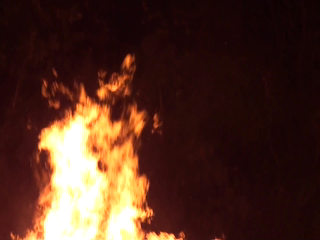
\includegraphics[width=0.5in]{stablefn/results/#1-#2/fr_00000.png} &
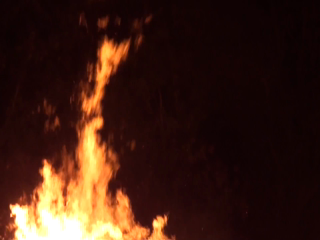
\includegraphics[width=0.5in]{stablefn/results/#1-#2/fr_00010.png} &
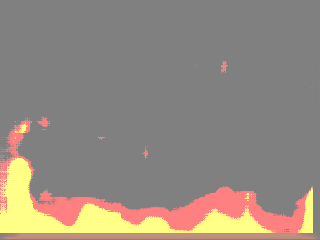
\includegraphics[width=0.5in]{stablefn/results/#1-#2/fr_00020.png} &
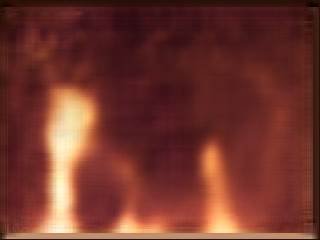
\includegraphics[width=0.5in]{stablefn/results/#1-#2/fr_00030.png} &
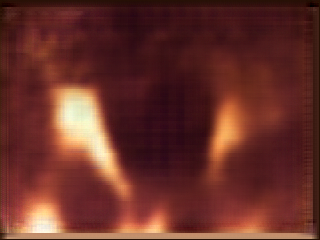
\includegraphics[width=0.5in]{stablefn/results/#1-#2/fr_00040.png} &
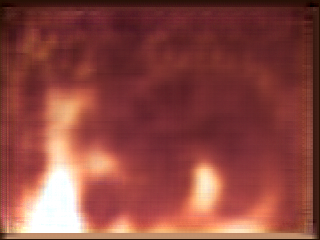
\includegraphics[width=0.5in]{stablefn/results/#1-#2/fr_00050.png} &
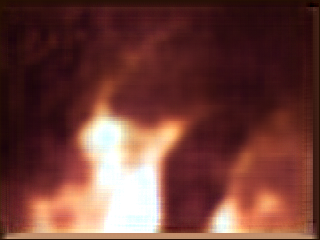
\includegraphics[width=0.5in]{stablefn/results/#1-#2/fr_00100.png} &
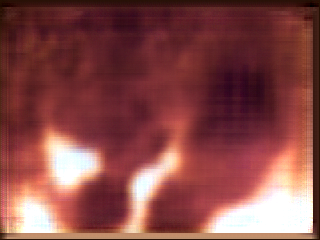
\includegraphics[width=0.5in]{stablefn/results/#1-#2/fr_00150.png} &
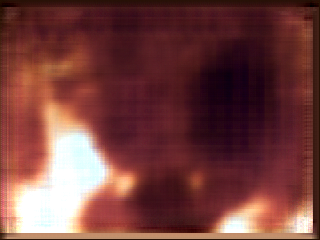
\includegraphics[width=0.5in]{stablefn/results/#1-#2/fr_00200.png} &
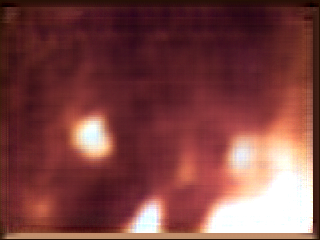
\includegraphics[width=0.5in]{stablefn/results/#1-#2/fr_00250.png}
}

\begin{tikzpicture}
    \begin{groupplot}[
        group style={
            group name=my plots,
            group size=5 by 1,
            horizontal sep=12pt
        },
        axis on top,% ----
        width=1.2in,
        height=1.2in,
        scale only axis,
        enlargelimits=false,
        xmin=0,
        xmax=1,
        ymin=0,
        ymax=1,
        axis x line*=bottom, axis y line*=left,
        ]

    \nextgroupplot[title={Stable Model Run 1},
    ytick={.1, 1},
    yticklabels={-2,18},
    xtick={.15, 1},
    xticklabels={$-10$,15}]
    \addplot[
        yticklabels={,,},
        xticklabels={,,}] graphics[xmin=-0.17,ymin=-0.17,xmax=1.17,ymax=1.17] {./stablefn/results/bonfire-exp27r-1e-5-1231132/trajmodel.png};

    \nextgroupplot[title={Stable Model Run 2},
    ytick={.1, 1},
    yticklabels={0,$20$},
    xtick={.15, 1},
    xticklabels={$0$,25}]
\addplot[] graphics[xmin=-0.17,ymin=-0.17,xmax=1.17,ymax=1.17] {./stablefn/results/bonfire-exp27r-1e-5-1238886/trajmodel.png};

    \nextgroupplot[title={Stable Model Run 3},
    ytick={.1, 1},
    yticklabels={-10,8},
    xtick={.1, .8},
    xticklabels={-5,15}]
    ]
    \addplot[] graphics[xmin=-0.17,ymin=-0.17,xmax=1.17,ymax=1.17] {./stablefn/results/bonfire-exp27r-1e-5-main/trajmodel.png};

    \nextgroupplot[title={Naive Model},
    ytick={.1, 1},
    yticklabels={0,},
    xtick={.1, 1},
    xticklabels={$-2 \times 10^{30}$,0},
        extra y tick labels={$1.2 \times 10^{30}$},
        extra y ticks={1.0},
        extra y tick style={y tick label style={right, xshift=0.25em}},]
    \addplot[] graphics[xmin=-0.17,ymin=-0.17,xmax=1.17,ymax=1.17] {./stablefn/results/bonfire-bad2/trajmodel.png};
    
    \nextgroupplot[
        ytick={0,1},
        yticklabels={0,300},
        ylabel={steps},
        width=.075in,
        axis line style={draw=none}, tick style={draw=none}, xticklabel=\empty, every axis y label/.style={at={(current axis.west)},rotate=90,yshift=-3mm,xshift=1mm},
        y tick label style={right, xshift=0.25em}]

    \addplot[] graphics[xmin=0,ymin=0,xmax=1,ymax=1] {./stablefn/viridis.png};

\end{groupplot}
\end{tikzpicture}
\begin{tabular}{r|cccccc|cccc}
Stable & \multicolumn{10}{c}{Frame Number} \\
Model & $0$ & ${10}$ & ${20}$ & ${30}$ & ${40}$ & ${50}$ & ${100}$ & ${150}$ & ${200}$ & ${250}$ \\
Run 1 &\sampletbl{bonfire}{exp27r-1e-5-main} \\
Run 2 &\sampletbl{bonfire}{exp27r-1e-5-1231132} \\
Run 3 &\sampletbl{bonfire}{exp27r-1e-5-1238886} \\
\shortstack{Naive\\Model} &
\sampletbl{bonfire}{bad2}
% \\ \shortstack{Sample\\Video} &    \sampletbl{bonfire}{sample}
\end{tabular}

  \caption{Samples generated by our stable video texture networks, with associated trajectories above. The true latent space is 320-dimensional; we project the trajectories onto a two-dimensional plane for display. For comparison, we present the video texture generated using an unconstrained dynamics model.}
  \label{fig:vae_results}
\end{figure}


\paragraph{Random networks. } To show that this construction learns provably stable networks we show the dynamics generated by a randomly initialized network in Figure~\ref*{fig:nominal_dynamics}. The three images show how a nominal dynamics function (left) is not inherently stable. A Lyapunov function following our construction (middle) is convex and positive definite, and the reprojection step generates dynamics that are stable (right).

\paragraph{Simple, damped pendulums. } This is trainable using any neural network framework with autodiff features, and doesn't require any specific loss function. When we train this model on simulated traces from a simple damped pendulum, we obtain the results in Figure~\ref*{fig:pendulum_experiment}. The simulated dynamics (left) are used to train our stable network, producing the dynamics (middle) and the lyapunov function (right). We separately verify that the learned Lyapunov function is consistent with the law of conservation of energy. To show the stability of this system, we further evaluate this on a range of n-link pendulums in Figure~\ref{fig:pendulum_results}. We see how the error of a naive model diverges with number of simulated steps and as the dynamics become more complex. The error of the stable model, however, \emph{decreases} as (due to energy loss from damping) the set of possible states the pendulum can exist in shrinks.

\paragraph{Video texture generation with VAEs. } Finally, we include a novel application of this in generating video textures, using a Variational Autoencoder (VAE) \citep{kingma2013auto} to learn an encoding from images to an encoding-space, and our stable network to learn a dynamics model in that encoding-space. We train these in an end-to-end manner to reconstruct the successor frame given the current frame of some video, minimizing both the standard VAE loss for the current frame and the reconstruction loss of the next generated frame. There is no specific loss function used to train the dynamics model.

To generate video textures, we seed the dynamics model with the encoding of a single frame and numerically integrate the dynamics model to obtain a trajectory, which is decoded into a sequence of frames. A small amount of additive random noise ensures that the trajectories don't collapse to zero. In Figure~\ref{fig:vae_results}, we present a sample of stable trajectories and frames produced by our network and compare it to an example trajectory generated by a naive dynamics model. The dynamics generated by the naive model quickly diverge and produce a fixed image, but our stable dynamics generate different trajectories that keep generating realistic images over long time horizons.

\subsubsection{Extension to stable policy and value functions. }

After the successes of our stable dynamics model, we attempted to use it to learn stable policies and value functions. The intuition is that we can replace the dynamics model $\hat f$ with fixed (known) dynamics $\tilde f$ and a learnable policy network $\pi$. That is, we train to minimize:
\begin{align}
  \mathsf{ReLU}\bigl(\nabla V(x)^T \tilde{f}(x, \pi) + \alpha V (x) \bigr)
\end{align}
given traces from simulated dynamics. We intended to learn stable value functions by manually setting a goal state and choosing a transformation for a Lyapunov function, and training it with TD learning from trajectory samples.

We find that we can learn stabilizing controllers for a one-link pendulum and the cartpole problem, but not a swingup controller for either or any type of controller for an Acrobot or more complex locomotion tasks. We could not overcome a particular type of training collapse where the learned Lyapunov function either collapses to a trivial function or the nominal dynamics function diverges to the point of uselessness\footnote{I have not seen any other method in the literature succeed in learning locomotion tasks with a large number of states using our stable-dynamics mechanism. }.

Given the failure of this method to generalize to stable control, we inferred that learning a stable value function was unlikely to succeed, and so shelved this line of inquiry.

\subsection{ODE stopping-time Policy and Value}

Learn dynamics and policies from trajectories using a novel ODE stopping-time formulation. One eventual goal was to learn policies that mimic expert trajectories and then iteratively improve the policy to increase the aggregate reward encountered during each trajectory. To do this we...\todo{Should we talk about the ODE stopping-time work? }

\section{Proposal: Projected Off-Policy TD (POP-TD) }

We propose an alternative approach to stabilizing off-policy training, inspired by Kolter's Non-Expansion Criterion and the original TD-DO algorithm \cite{kolter2011fixed}. 
In this approach, Kolter proposes selecting a convex set of ``safe'' distributions and reweighting data so it appears to come from such a distribution. The resultant algorithm is called Projected Off-Policy TD (POP-TD).

Even though POP-TD and Emphatic-TD both resample distributions, there are three key differences between them:
\begin{enumerate}
  \item the distribution after reweighting in POP-TD is provably non-expansive, but not necessarily the on-policy distribution (as enforced by Emphatic-TD). This allows POP-TD much greater flexibility in training
  \item POP-TD is not vulnerable to the regularization pitfalls explained in Section~\ref{sec:rr}.
  \item POP-TD is not prone to the same high-variance updates as the followon trace model in Emphatic-TD.
\end{enumerate}
We introduce Kolter's Non-Expansion Criterion, and then explain how our proposed project extends this.

%%%%%%%%%%%%%%%%%%%%%%%%%%%%%%%%%%%%%%%%%%%%%%%%%%%%%%%%%%%%
\subsection{Background }

There is some work in the literature on which our methods rely. We cover the appropriate background here:

\subsubsection{Kolter's Non-Expansion Criterion }

Kolter's Non-Expansion Criterion was introduced by Kolter in \citeyear{kolter2011fixed}. The core idea is to estimate a convex set of ``safe'' distributions, under which TD updates are guaranteed to be non-expansive despite an off-policy update projection. To do this, he writes down this inequality concerning the $D$-norm of the learned value function the Bellman update, where $D=\text{diag}(\mu)$:
\begin{align}
    \|\Pi_D P\Phi \vec w\|_D & \leq \|\Phi \vec w\|_D
\end{align}
This is true if and only if the matrix $F_D$ is positive semi-definite
\begin{align}
    F_D \equiv & \begin{bmatrix}
        \Phi^\top D \Phi & \Phi^\top D P \Phi \\
        \Phi^\top P^\top D \Phi & \Phi^\top D \Phi
    \end{bmatrix} \succcurlyeq 0 \label{eqn:koltercondmat}
\end{align}
This can be written in terms of an expectation over the sampling distribution $\mu$. Let $\mu : \mathcal S \to \mathbb R^+$ be the PDF of state $s \in \mathcal S$, and the transition distribution $p(s,s') = \mu(s) p(s'|s)$. (We also assume that $\mu(s) > 0 \quad (\forall s)$ -- this is called the \emph{full-coverage} assumption.) This condition is equivalent to:
\begin{align}
  \E_{s\sim \mu, s'\sim p(s'|s)} & \left[\begin{bmatrix}
        \phi(s)\phi(s)^\top & \phi(s)\phi(s')^\top \\
        \phi(s')\phi(s)^\top & \phi(s)\phi(s)^\top
    \end{bmatrix}\right] \succcurlyeq 0 \label{eqn:koldercondstate}
\end{align}
For convenience, we write down the per-state contribution to this expectation as:
\begin{align}
F(s) = \E_{s'\sim p(s'|s)} & \left[\begin{bmatrix}
    \phi(s)\phi(s)^\top & \phi(s)\phi(s')^\top \\
    \phi(s')\phi(s)^\top & \phi(s)\phi(s)^\top
\end{bmatrix}\right]
\end{align}
This allows us to write Equation~\ref{eqn:koldercondstate}:
\begin{align}
\E_{s\sim \mu} & [F(s)] \succcurlyeq 0
\end{align}
In practice this condition does not always hold at $\mu$. We can apply this insight to data by reweighting incoming samples so they are consistent with a different distribution $q$ such that
\begin{align}
\E_{s\sim q} & [F(s)] \succcurlyeq 0
\end{align}
For input data $(x_1, x_2, \ldots)$, this is the same as finding a set of weights $q_1, q_2, \ldots$ such that
\begin{align}
\sum_i q_i & \cdot F(x_i) \succcurlyeq 0
\end{align}
We also need to constrain our choice of distribution $q$ to ensure the quality of the solution. \citet{kolter2011fixed} achieve this by selecting $q$ that solves this optimization problem
\begin{align}
    \underset{q}{\text{minimize}}~\text{KL}(\mu||q) & \qquad \text{s.t. } ~ E_{s\sim q}[F(s)] \succcurlyeq 0 \label{eqn:kolter2011objective}
\end{align}
explicitly optimizing over the distributons using a primal-dual formulation that exploits the structure of the problem. The resultant algorithm, TD-DO, performs a first-order optimization method on a dual objective using quasi-Newton methods alongside every TD step.


\subsubsection{I- and M-projections} \label{sec:improj}
The Kullback-Leibler divergence is an \emph{asymmetric} measure, and so it is usually the case that $\min_q~\text{KL}(q||\mu) \neq \min_q~\text{KL}(\mu||q)$. The former (``from $\mu$ to $q$'') is an information (or I-)projection, which tends to under-estimate the support of $q$ potentially excluding possible sampling distributions to reweight to. The latter (``from $q$ to $\mu$'') is a moment (or M-)projection, which tends to over-estimate the support of $q$ and avoid zero solutions. In our solution, we are proposing using an I-projection instead of the M-projection used by \citet{kolter2011fixed}. 

\subsubsection{Offline/Batch RL}

Offline RL is a field of RL which focuses on learning optimal policies from a static dataset sampled from an unknown policy, possibly a policy designed for a different task. In offline RL, algorithms are expected to learn entirely from environment samples without the ability to interact with the environment. This is commonly useful to learn in environments that are expensive to explore in (such as running a Tokamak nuclear reactor), or in extremely high-dimensional environments with cheap access to expert trajectories (such as video games). \citet{levine2020survey} present a comprehensive survey of the area.

The key difference is that, in offline RL, the data is not gathered interactively. This leads to several problems, most notably \emph{distribution shift} (or \emph{distributional mismatch}), in which the distribution implied by the learned policy is very different from the distribution of the data included. This is well-understood in the literature that the source of this error is from bootstrapping outside the support of the dataset, and solutions generally work by constraining the learned policy in some manner. \citet{fujimoto2019off} constrain the action space to prevent straying from sampling policy, which is improved on by BEAR \cite{kumar2019stabilizing} which allows learned policies to stray from the sampling policy under limited conditions. \citet{laroche2019safe} interpolate bootstraps from the learned policy or the sampled data, depending on the uncertainty of the value.

Some approaches leverage a dynamics model that is also learned from the data: MOPO \cite{yu2020mopo} use ensembles to understand the epistemic uncertainty of the dynamics around states and penalize the value estimates of more uncertain states, \cite{tianhe2021combo} eschew explicit uncertainty modeling by penalizing out-of-support data generated by their dynamics models. By constraining the model to be no better than the original environment, MoREL \cite{kidambi2020morel} learns a surrogate MDP that they can optimize over with an online RL algorithm. More unusual methods devise entirely different RL algorithms to address this. In particular, Advantage-weighted Regression \cite{peng2019advantage} decomposes the problem into individual components that are learnt in a supervised manner.

This area is natural application for our method. Naive methods are known to require exponentially many samples (in the problem horizon) to resolve distribution shift \cite{wang2020statistical}, and our method may help reduce this requirement. Many existing methods are limited because they over-constrain the learned policies to prevent runaway self-reinforcement outside the support of the data. In contrast, using our method to reweigh samples to a regular RL algorithm guarantees that the resultant model is not vulnerable to this.


\subsection{Our Algorithm}
A deceptively simple theoretical insight opens up a new algorithmic possibility. Instead of the M-projection objective in Equation~\ref{eqn:kolter2011objective}, we optimize the dual I-projection instead:
\begin{align}
  \underset{q}{\text{minimize}}~\text{KL}(q||\mu) & \qquad \text{s.t. } ~ E_{s\sim q}[F(s)] \succcurlyeq 0 \label{eqn:ouroptobj}
\end{align}
By changing the objective, we are able to integrate its solution into the basic TD algorithm and solve these concurrently. This avoids the first-order optimization in each update step, greatly reducing the time-complexity of the resultant algorithm. By switching to an I-projection, we may even improve the quality of the closest distribution $q$.

The dual of (\ref{eqn:ouroptobj}) can simplified to 
\begin{align}
  \underset{Z \succcurlyeq 0}{\text{minimize}}~\E_\mu [\exp(\text{tr} Z^\top F(s))] \label{eqn:ouroptobjdual}
\end{align}
where $Z$ is a Lagrange multiplier. We assume (and later verify) that $Z$ is low-rank and follows the structure
\begin{align}
  Z & = \begin{bmatrix}
    Z_0 & - Z_0 \\ -Z_0 & Z_0
  \end{bmatrix}
\intertext{which we approximate as a rank-one solution with parameters $y\in \mathbb{R}^{k}$ following the Burer-Monteiro approach}
  Z & = \begin{bmatrix} y \\ -y \end{bmatrix}
  \begin{bmatrix} y \\ -y \end{bmatrix}^\top
\end{align}
Substituting this into Equation~\ref{eqn:ouroptobjdual}, this objective simplifies to the unconstrained optimization problem
\begin{align}
  \underset{y}{\text{minimize}}~\E_\mu [\exp(y^\top A(s) y)] \quad\text{where~} A(s) = \E_{s\sim\mu,s'\sim p(s'|s)} [\phi(s)(\phi(s) - \phi(s'))^\top] \label{eqn:outoptobjunconstr}
\end{align}
To solve this problem in linear time we adopt a two-timescales method, separately estimating $y$ and $(y^\top A(s) y)$. To minimize the memory overhead, we directly represent $y \in \mathbb R^{k}$ (which is the same size as the learned weights), but approximate $g_\theta(s) = (y^\top A(s) y)$ using a separate function approximator with parameter $\theta$.

Differentiating the objective in Equation~\ref{eqn:outoptobjunconstr} with respect to $y$, we obtain:
\begin{align}
  \nabla_y \mathbf{E}_\mu \left [ \exp (y^T A(s) y) \right ] & = 
  \E_{s \sim \mu, s' \sim p(\circ|s)} \left [ \exp(2 g_\theta(s)) \phi(s)(\phi(s) - \phi(s'))^T y \right ]
\intertext{From this, at each step of the underlying TD algorithm, we drive each parameter towards the objective values:}
  g_\theta(s) & \to (\phi(s)^\top) y \cdot (\phi(s)^\top - \phi(s')^\top) y \\
  y & \to \exp{g_\theta(s)} (\phi(s)^\top - \phi(s')^\top) y \cdot \phi(s)
\intertext{This may require tinkering with the update rates (or using a target network construction) or other implementation tricks to ensure training stability. Alongside these two update rules, we augment the TD update to reweigh each sample:}
  w & = w - \alpha \exp(2 g_\theta(s)) (\phi(s)^\top w - r - \phi(s')^\top w) \cdot \phi(s) 
\end{align}

\subsection{Preliminary Results }

We have a preliminary implementation of this algorithm to verify its basic function. We conduct the initial tests of our algorithm on three toy examples, designed to characterize the performance of the algorithm as we sample off-policy.

%%
\begin{figure}[t]
  \begin{tikzpicture}
    \begin{axis}[
        scale only axis,
        width=\textwidth-10mm,
        height=5cm,
        tick align=outside,
        enlargelimits=false,
        ymode=log,
        mark=none,
        ymax=10,
        xlabel={$p$ in sampling distribution $\mu=[\sfrac p2, \sfrac p2, 1-p]$},
        yticklabels={,,},
        ylabel={TD error},
    ]
    \addplot[color=viridis09,thick] table [x=p, y=err] {thesiswork/threestate/eta_-infty.dat} node[above,pos=0.99] {Naive TD};
    \addplot[color=viridis03,thick] table [x=p, y=err] {thesiswork/threestate/export_threestate.dat} node[above,pos=0.7] {POP-TD};
    \end{axis}
\end{tikzpicture}

  \caption{We plot the error of various TD methods against $p$ for three-state MDP from \cite{manek2022pitfalls}. The on-policy distribution is at $p=0.5$, and Kolter's non-expansion criterion is met in the domain $p\in[0, 0.5]$. We see that naive TD diverges around $p\approx0.71$, but POP-TD retains low error in that region. }
  \label{fig:prelimthreestate}
\end{figure}
%%


\paragraph{Three-state MDP} First, we present the performance at convergence on the three-state example from \cite{manek2022pitfalls}. This example is a simple three-state MDP with well-understood divergence. In Figure~\ref{fig:prelimthreestate}, we plot the effect of using naive TD and observe the characteristic divergence at about $p=0.71$. Running our implementation of POP-TD (until convergence, with a batch size of 32 and a large learning rate) we obtain the second plot in that figure.


Recall that our algorithm reweights TD updates to the closest distribution in which Kolter's non-expansion criterion is met. This corresponds to the domain $p\in[0, 0.5]$ in the three-state example. This explains why the error curve from POP-TD exactly follows naive TD in the domain $p\in[0, 0.5]$, because no reweighting is necessary. Further, distributions in the domain $p\in(0.5, 1]$ are all mapped to the closest distribution $p=0.5$--where the error is the lowest--and so POP-TD exhibits that low error in the right half of the plot. Around $p=1.0$ error increases sharply because that distribution violates the full-coverage assumption (that the support of the sampling distribution covers all states in the closest distribution).

\paragraph{Diffusion and Random MDPs} We further test POP-TD on the advanced tasks in \cite{kolter2011fixed}: the randomly-generated MDP and randomly-generated diffusion chain. Following the procedures described in the paper, we generate both MDPs and find the value function using both vanilla TD and POP-TD with similar parameters. As in the previous work, we plot the performance of both as a function of training.




\subsection{Remaining Work }

The proposed project is to complete the design of POP-TD, evaluate it across a range of problems, and (if possible) prove its correctness, convergence, and performance.

\subsubsection{Full Implementation and Evaluation }

The natural application for this is in the field of offline RL.
\todo{Why?}

\begin{enumerate}
  \item Implement with stochastic updates
  \item Evaluate on a sequence of tasks:
  \begin{enumerate}
    \item Toy examples (Online RL)
    \begin{enumerate}
      \item Three-state
      \item Diffusion chain/Random MDPs
    \end{enumerate}
    \item Locomotion examples (Offline RL)
    \begin{enumerate}
      \item Cartpole
      \item Lunar Lander
    \end{enumerate}
    \item Atari-like examples (Offline RL)
    \begin{enumerate}
      \item Maze2D
      \item ???
    \end{enumerate}
  \end{enumerate}
\end{enumerate}


\subsubsection{Our Assumption that the Lagrange Multiplier is Low-Rank }

In our algorithm, we make a three-step structural assumption on $Z$. We first assume that $Z$ has this special block structure:
\begin{align}
  Z & = \begin{bmatrix}
    Z_0 & - Z_0 \\ -Z_0 & Z_0
  \end{bmatrix}
\intertext{and then we further assume that the solution follows the Burer-Monteiro approach:}
  Z & = \begin{bmatrix} Y \\ -Y \end{bmatrix}
  \begin{bmatrix} Y \\ -Y \end{bmatrix}^\top
\intertext{and then we finally assume that the solution has rank one:}
  Z & = \begin{bmatrix} y \\ -y \end{bmatrix}
  \begin{bmatrix} y \\ -y \end{bmatrix}^\top
\end{align}

We observe that this holds in all our toy examples: three-state, diffusion-chain, and random MDPs. To verify this, we solve an SDP representing Equation~\ref{eqn:ouroptobjdual} and obtain an optimal $Z$ without any rank constraint. We verify that the $Z$ we obtain follows Burer-Monteiro, and we then verify that the rank-one approximation of the component $Z_0$ can recover the original $Z$ (permitting a small amount of floating-point error). As a secondary check, we verify that the $Z$ reconstructed from the rank-one approximation represents a valid solution that, when used to remap TD updates, renders them non-expansive.

\paragraph{Note:}
We are not investigating the claim that some rank-one solution minimizes Equation~\ref{eqn:ouroptobjdual}. We are instead investigating the stronger assumption that the solution (of any possible rank) that minimizes Equation~\ref{eqn:ouroptobjdual} always has a rank one approximation.

There is no clear reason why this should be true, but we have two possible avenues of investigation: first, we have a set of counterexamples invented for \emph{Pitfalls} \cite{manek2022pitfalls} that are known to be pathological by having negative or zero eigenvalues in the corresponding $F$-matrix. If the rank of the solution is related to the number of negative eigenvalues of $\E_{s\sim\mu} [F(s)]$, then one of those may provide a counterexample and also shed light on the reason behind the structure of $Z$. Second, we know from the KKT conditions of the related optimization problem in \cite{kolter2011fixed} that the rank of $Z$ and $F$ are complementary -- if we can prove the property also holds here, it may be sufficient to find the conditions under which $F$ is full rank. In any case, this is an easily testable hypothesis.

Our goal is to understand \emph{why} this property has held so far and achieve one of the following:
\begin{enumerate}
  \item prove that it must always hold,
  \item find an example where the optimal $Z$ does not admit a rank-one approximation that also satisfies the problem, or
  \item reduce this to an existing unsolved problem.
\end{enumerate}

\subsubsection{Prove convergence of POP-TD}

We wish to prove that our two-timescales structure (learning $y$ and $g(s) = y^\top A(s) y$ separately) and update rules are such that these two functions will converge a solution. Assuming a fixed sampling policy (and with additional mild assumptions), we wish to show that the update rules form a dynamical system that is convergent.

Unlike in online RL, the dataset does not vary with the policy we learn and so the data distribution is fixed. This means we do not need to consider the effects of a changing sampling distribution on the convergence of our algorithm. We may extend our analysis by attempting to prove that it remains well-behaved even in the context of a slowly changing sampling distribution (as in \cite{zhang2021breaking}), which would allow us to recommend this algorithm for online TD learning as well.


\subsubsection{(Optionally) Bound the quality of the solution at convergence. }

A particularly difficult ``stretch'' goal is to prove bounds on the quality of the solution reached by POP-TD. From other examples in the literature \cite{zhang2020provably,zhang2021breaking}, we know that these bounds are likey to be loose in pathological cases, but the structure of the derived bounds would be an exciting result.

We may first derive bounds with the simplifying assumption that $g : \mathcal S \to mathbb R$ is tabular, as that prevents the chicken-and-egg problem of $g$ itself being vulnerable to instability from off-policy training. (The version of Emphatic-TD we analyzed in \ref{sec:rr} has such a vulnerability.)


\clearpage

\printbibliography

\clearpage

\appendix
%\section{Appendix }

\section{Technical Details}

This is a complete derivation of the theory behind this project, starting from Kolter's non-expansion condition \cite{kolter2011fixed} and ending with the production of the update rules. This is an elaborated version of \cite{kolternote2022}.

\subsection{Kolter's non-expansion condition}

Error bounds from on-policy TD follow the property that the $\diag(\pi)-$norm of any vector $x \in \mathbb R^n$ is non-expansive through the transition matrix. That is: $\|Px\|_{\diag(\pi)} \leq \|x\|_{\diag(\pi)}$.  \citep{kolter2011fixed}, observes that we can relax this to potentially off-policy distributions $D$. He writes down \emph{Kolter's non-expansion condition}:
\begin{align}
  \|\Pi_D P\Phi \vec w\|_D & \leq \|\Phi \vec w\|_D \qquad (\forall w \in \mathbb R^n)
\intertext{This holds if and only if the matrix $F_D$ is positive semi-definite}
F_D \equiv & \begin{bmatrix}
  \Phi^\top D \Phi & \Phi^\top D P \Phi \\
  \Phi^\top P^\top D \Phi & \Phi^\top D \Phi
\end{bmatrix} \succcurlyeq 0
\end{align}
This constraint describes a convex subset of $D$. As a $2k\times 2k$ matrix (where $k$ is the number of features), $F$ is prohibitively large to enumerate for any real RL problem, and so our algorithm is designed to make use of this without ever constructing it directly. Further, we notice that the construction of $F_D$ depends on $P$, the transition matrix of the underlying Markov process, which complicates how we construct it from samples.

Later in the algorithm, we will need to compute the contribution of a single sample to the expectation of $F$. To do this, we define the function $F(s, s')$ as the contribution of a single state-transition pair towards the construction of $F_D$. That is:
\begin{align}
  F(s, s') & = \begin{bmatrix}
    \phi(s)\phi(s)^\top & \phi(s)\phi(s')^\top
\\  \phi(s')\phi(s)^\top & \phi(s)\phi(s)^\top
  \end{bmatrix}
\intertext{and its expectation:}
F_{\diag(\mu)} & = \E_{s\sim \mu, s'\sim p(\circ|s)} F(s, s')
\intertext{For convenience, we define the shorthand $F(s)$, noting that it depends on the transition distribution $p(\circ|s)$.}
  F(s) & = \E_{s'\sim p(\circ|s)} F(s, s')
\end{align}

Directly constructing $F(s)$ or $F(s, s')$ is impossible on all but the simplest examples -- it would take $\mathcal O(k^2n)$ memory to hold all the necessary data. Instead we exploit the structure inherent in the problem to make use of $F(s)$ without creating it .


\subsection{Optimizing the distribution}

In the previous section we have characterized a convex subset of off-policy distributions under which TD learning is guaranteed not to diverge. If we can discover any such distribution for a particular TD problem, we can reweigh our TD updates (from any distribution) so they appear consistent with this reweighting distribution. This is related to the main insight in Emphatic-TD \cite{sutton2016emphatic}, with the key innovation that we can take any non-expansive distribution, \emph{not just the on-policy distribution}.

We can now write down the optimization problem that we wish to solve: 
\begin{align}
  \underset{q}{\text{minimize}}~\text{KL}(q||\mu) & \qquad \text{s.t. } ~ E_{s\sim q}[F(s)] \succcurlyeq 0
\end{align}
We are searching for $q$, the closest distribution to the sampling distribution $\mu$ such that $F$ is PSD under $q$. Note that we could in principle minimize any notion of ``closest'' to find some satisfying distribution -- for example \citet{kolter2011fixed} explores the effects of minimizing $\text{KL}(\mu||q)$.

We construct the dual of this problem:
\begin{align}
  \underset{Z\succcurlyeq 0}{\text{maximize}}~ \underset{q}{\text{minimize}}~\text{KL}(q||\mu) - \tr Z^\top \E_{s\sim q}[F(s)]
\end{align}
Using the Lagrange multiplier $Z\in\mathbb R^{2k\times 2k}$, we solve the inner optimization problem:
\begin{align}
  \underset{q}{\text{minimize}} - H(q) - \E_{s\sim q}[\log \mu(s) + \tr Z^\top F(s)]
\end{align}
Writing down Lagrangian and solving for the optima, we obtain:
\begin{align}
  q^*(s) & \propto \mu(s)\exp( \tr Z^\top F(s))
\end{align}
(Subject to the constraint that $q^*(s)$ is normalized so it must sum to 1 over all $s$.)

Plugging this back into our dual formulation, we obtain the optimization problem:
\begin{align}
  \underset{Z\succcurlyeq 0}{\text{maximize}} & -\log \E_{s\sim\mu} [ \exp(\tr Z^\top F(s)) ]
\intertext{Which we can simplify to}
\underset{Z\succcurlyeq 0}{\text{minimize}} & \E_{s\sim\mu} [ \exp(\tr Z^\top F(s)) ]
\end{align}

As discussed earlier, $F(s)$ cannot be directly constructed; instead, we assume that $Z$ holds a specific structure and optimize the problem.


\subsection{Simplifying the optimization problem}

Our next goal is to transform this constrained optimization problem into an unconstrained problem over a low-rank version of $Z$, suitable for learning via SGD.

We assume (and later check!) that the solution for $Z$ is low-rank. Intuitively, this is because $\E_{s\sim\mu}[F(s)]$ is PSD when $\mu$ is close to $\pi$, and for most MDPs, sampling off-policy leads to only a small number of negative eigenvalues that need to be corrected by $Z$. \citet{kolter2011fixed} provide a technical explanation: by the KKT conditions, $Z$ will have rank complementary to $\E_{s\sim\mu}[F(s)]$, and the latter is expected to be full rank. It is worth noting that this ``almost-PSD'' assumption is common in the field, is supported by the work in \cite{manek2022pitfalls}. We later discuss how we verify that this assumption holds.

We make the strong assumption that $Z$ is rank one, and apply the Burer-Montiero \todo{cite} approach to convert the constrained optimization problem over $Z$ into an unconstrained optimization over $y\in \mathbb R^{k}$:
\begin{align}
  Z^\star & = \begin{bmatrix} y \\ -y \end{bmatrix} \begin{bmatrix} y \\ -y\end{bmatrix}^T
\end{align}
Substituting this into the dual formulation, we get:
\begin{align}
\underset{y}{\text{minimize}} & \;\; \mathbf{E}_{s\sim\mu} \left [ \exp\left (\tr  \begin{bmatrix} y \\ -y \end{bmatrix} \begin{bmatrix} y \\ -y\end{bmatrix}^T F(s) \right )  \right ]
\end{align}

We can leverage the structure of $F(s)$ to simplify the trace term:
\begin{align}
\tr  \begin{bmatrix} y \\ -y \end{bmatrix} \begin{bmatrix} y \\ -y \end{bmatrix}^T F(s)
    & = \begin{bmatrix} y \\ -y \end{bmatrix}^T F(s) \begin{bmatrix} y \\ -y \end{bmatrix} \\
\\  & =  \begin{bmatrix} y \\ -y \end{bmatrix}^T  \mathbf{E}_{s' \sim p(s'|s)}  \left[ \begin{array}{cc} \phi(s)\phi(s)^T & \phi(s)\phi(s')^T \\ \phi(s')\phi(s)^T & \phi(s)\phi(s)^T \end{array} \right]
 \begin{bmatrix} y \\ -y \end{bmatrix} \\
\\  & =  2 y^T \mathbf{E}_{s' \sim p(s'|s)} \left [\phi(s)(\phi(s)- \phi(s'))^T \right ] y
\\  & =  2 y^T A(s) y
\end{align}
where $A(s) = \mathbf{E}_{s' \sim p(s'|s)} \left [\phi(s)(\phi(s)- \phi(s'))^T \right ]$

This allows us to rewrite the optimization problem as:
\begin{align}
  \underset{y}{\text{minimize}} & \;\; \mathbf{E}_{s\sim\mu} \left [ \exp\left(2 y^\top A(s) y \right)  \right ]
\end{align}

This has some great properties: in particular, we can optimize $y$ in an unconstrained manner (i.e. with SGD), and we need only use quantities that we already compute ($\phi(s), \phi(s')$). All this leads to the final step, the derivtion of the update rules:


\subsection{Update rules}

We can't directly optimize $y$ because that would require us to create $A(s)$. Instead, we use a two-timescales approach by estimating two (dependent) quantities separately and improving them at potentially different rates. By optimizing over the two quantities simultaneously, we hope to be able to discover the convergent value. This is generally possible with a little tuning.

We choose to optimize $y \in \mathbb R^k$ which is the same size as $w$, and the trace estimate $g(s) = y^\top A(s) y \in \mathbb R^n$. Instead of learning a tabular $g(s)$, we can approximate it as a linear function (or a neural network, for larger problems). This decision means the size of the per-update weights are still $\mathcal O(k)$ (limited by $w$ and $y$).

We find the derivative of the objective with respect to $g(s)$ and $y$ and use that to construct update rules for our algorithm.
\begin{align}
  \nabla_y \mathbf{E}_\mu \left [ \exp (2 y^T A(s) y) \right ] & = 
  \mathbf{E}_{s \sim \mu(s)} \left [ \exp (2 y^T A(s) y) \; A(s) y \right ]
\\  & = \mathbf{E}_{s \sim \mu(s), s' \sim p(s'|s)} \left [ \exp (2 y^T A(s) y) \; \phi(s)(\phi(s) - \phi(s))^T y \right ]
\intertext{We substitute $g(s)$ into this to arrive at the final gradient derivation}
    & = \mathbf{E}_{s \sim \mu(s), s' \sim p(s'|s)} \left [ \exp(2 g(s)) \; \phi(s)(\phi(s) - \phi(s'))^T y \right ].
\end{align}

This corresponds to the update rules:
\begin{align}
  a & := \phi(s)^\top y \\
  b & := \phi(s')^\top y \\
  \theta & := \theta - \alpha_1 (g_\theta(s) - a(a-b))\nabla_\theta g_\theta(s) \\
  y & := y - \alpha_2 \exp(2 g_\theta(s)) (a-b) \phi(s)
\end{align}
where $\theta$ is the parameterization of $g(s)$, and $\alpha_\circ$ are learning rates.

And finally, to complete this, we multiply each update of $w$ by $\exp(2 g(s))$ to resample it so it appears to come from the ``safe'' distribution, which completes the description of the algorithm!



\end{document}
